\chapter{トレースログ可視化ツール TraceLogVisualizer の利用}

\if0
\section{トレースログの可視化}
本節では,開発したTLVを用いて,様々な形式のトレースログの可視化を行い,汎用性があることを確認する.

まず,シングルコアプロセッサ用RTOSの可視化を行い,動作の確認を行う.
次に,マルチコアプロセッサ用RTOSの可視化に対応するように拡張し,どの程度の作業で拡張が行えるのかを確認する.
最後に,組込みコンポーネントシステムの可視化を行い汎用性の確認を行う.
\fi

\section{シングルコアプロセッサ用RTOSのトレースログの可視化}
可視化するシングルコアプロセッサ用RTOSとして,TOPPERS/ASPカーネルを用いた.TOPPERS/ASPカーネルは,標準でトレースログを取得する機能を搭載しており,カーネルの動作開始と終了,処理単位の実行開始と終了,タスク状態の変化,ディスパッチャの実行開始と終了,サービスコールの入口と出口といった情報をトレースログ取得できる.
処理単位とは,割込みハンドラ,割込みサービスルーチン,周期ハンドラ,アラームハンドラ,CPU例外ハンドラ,タスク例外処理ルーチンを指す.

TOPPERS/ASPカーネルのトレースログの例は表\ref{aspTraceLog}で示している.

任意の形式をもつトレースログをTLVで可視化表示するために必要な作業は,可視化表示する項目の決定,リソースヘッダファイルの記述,変換ルールファイルの記述,,可視化ルールファイルの記述である.

また,TLVでは,トレースログに含まれるリソースをリソースファイルとして定義し,読み込まなければならないため,リソースファイルを記述する作業も必要になる.

\subsection{可視化表示する項目の決定}
\label{subsec414}

可視化表示する項目は,タスクの状態遷移,システムコールとした.

タスクの状態遷移の可視化表現は,実行状態を緑色の四角形,実行可能状態を黄色い線分,待ち状態を赤い線,起動を上矢印,終了を下矢印とする.
図\ref{fig:taskStateChangeVisual}にタスクの状態遷移の可視化表現の例を示す.

システムコールの可視化表現は,赤色の四角形で,枠線を点線,高さを待ち状態の線と同じ高さとする.
このとき,システムコール名,システムコールの引数を四角形の上左隅,返値であるエラーコードを下右隅に文字列で出力するとする.
図\ref{fig:svcCallVisual}にシステムコールの可視化表現の例を示す.

\begin{figure}[t]
\begin{center}
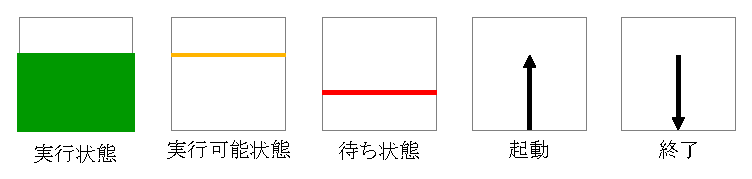
\includegraphics[scale=0.75]{img/taskStateChangeVisual.eps}
\caption{タスクの状態遷移の可視化表現例}
\label{fig:taskStateChangeVisual}
\end{center}
\end{figure}

\begin{figure}[t]
\begin{center}
\includegraphics[height=3cm]{img/svcCallVisual.eps}
\caption{システムコールの可視化表現例}
\label{fig:svcCallVisual}
\end{center}
\end{figure}

\subsection{リソースヘッダファイルの記述}

前述の可視化表示はタスクの挙動に関してであるので,リソースタイプとしてはタスクを定義すればよい.

表\ref{aspTraceLog}によると,トレースログ内においてタスクはタスクIDを指定して記録されている.
また,状態の遷移を可視化表示したいため,タスクの属性としては,タスクIDと状態を考慮すればよい.

前述の可視化表現を描画するためには,以下のようなイベントを標準形式トレースログで出力しなければならない.
そのため,それぞれを振る舞いとして定義する.

\begin{itemize}
\setlength{\itemsep}{-2mm}
\item システムコールに入った
\item システムコールから出た
\item タスクが起動した
\item タスクが終了した
\end{itemize}

タスクのリソースタイプを{\tt Task}として表\ref{resourceTypeTask}のようにリソースヘッダファイルに定義した.

\begin{File}{TOPPERS/ASPカーネル用リソースヘッダファイル}{resourceTypeTask}
{
  "asp":
  {
    "Task":{
      "DisplayName":"タスク",
      "Attributes":{
        "id":{
          "VariableType"  :"Number",
          "DisplayName"   :"ID",
          "AllocationType":"Static",
          "CanGrouping"   :false
        }
        "state":{
          "VariableType"  :"String",
          "DisplayName"   :"状態",
          "AllocationType":"Dynamic",
          "CanGrouping"   :false,
          "Default"       :"DORMANT"
        }
      },
      "Behaviors"  :{
        "activate":{
          "DisplayName":"起動"
        }
        "exit":{
          "DisplayName":"終了"
        }
        "enterSVC":{
          "DisplayName":"サービスコールに入る",
          "Arguments"  :{
            "name":"String",
            "args":"String"
          }
        },
        "leaveSVC":{
          "DisplayName":"サービスコールから出る",
          "Arguments"  :{
            "name":"String",
            "args":"String"
          }
        }
      }
    }
  }
}
\end{File}

前述のシステムコールの可視化表現では,システムコールの名前と引数,返値のエラーコードを文字列として出力したいため{\tt enterSVC}と{\tt leaveSVC}に引数としてそれらを指定するようにした.

\subsection{変換ルールファイルの記述}

表\ref{aspTraceLog}で示したTOPPERS/ASPカーネルのトレースログを標準形式トレースログに変換するための変換ルールファイルを記述する.

タスクの状態変化の可視化表示には,リソースタイプ{\tt Task}の属性{\tt state}が変わったという属性変化イベントと,振る舞い{\tt activate()}と{\tt exit()}が発生したという振る舞いイベントをイベント期間として指定すればよい.

TOPPERS/ASPカーネルのトレースログは,タスクの状態遷移を表\ref{aspTaskStateChangeTraceLog}のような形式で表現している.

\begin{table}[p]
\begin{quote}
\begin{breakbox}
{\tt [}{\it time}{\tt ] task }{\it taskId}{\tt \ becomes }{\it state}{\tt .}
\end{breakbox}
\caption{TOPPERS/ASPカーネルのトレースログにおけるタスクの状態遷移を表す形式}
\label{aspTaskStateChangeTraceLog}
\end{quote}
\end{table}

{\it time}は時間であり,時間の単位はマイクロ秒である.
{\it taskId}はタスクIDを,{\it state}は遷移後の状態を表している.

この形式に一致した際に出力するべき標準形式トレースログを表\ref{aspTaskStateChangeStandardTraceLog}に示す.

\begin{table}[p]
\begin{quote}
\begin{breakbox}
{\tt [}{\it time}{\tt ] Task(id==}{\it taskId}{\tt ).state=}{\it state}
\end{breakbox}
\caption{タスクの状態遷移を表す標準形式トレースログ}
\label{aspTaskStateChangeStandardTraceLog}
\end{quote}
\end{table}

しかし,TOPPERS/ASPカーネルでは,実行状態と実行可能状態を内部では状態として区別しておらず,{\tt RUNNING}への遷移と,{\tt RUNNABLE}から{\tt RUNNING}への遷移を上記の形式で記録しない.
そのため,上記の形式のトレースログでタスクの状態遷移のすべてを標準形式トレースログで出力するのは不可能である.

TOPPERS/ASPカーネルでは,タスクが実行状態になったかどうかを表\ref{aspTaskStateBecomeRunningTraceLog}のような形式のトレースログで記録する.

\begin{table}[p]
\begin{quote}
\begin{breakbox}
{\tt [}{\it time}{\tt ] dispatch to task }{\it taskId}{\tt .}
\end{breakbox}
\caption{TOPPERS/ASPカーネルのトレースログにおけるタスクが実行状態になったことを表す形式}
\label{aspTaskStateBecomeRunningTraceLog}
\end{quote}
\end{table}

これは,ディスパッチャから出てタスクIDが{\it taskId}のタスクの実行に遷移したことを表している.
この形式のトレースログによりタスクが{\tt RUNNING}へ遷移したことを標準形式トレースログで出力する.
また,{\tt RUNNABLE}から{\tt RUNNING}への遷移は,この形式のトレースログに一致した際に,時刻がそのトレースログの{\it time}のときに状態が{\tt RUNNING}のタスクが存在する場合に,そのタスクを{\tt RUNNABLE}へ遷移したことを標準形式トレースログで出力することで行う.

タスクの起動の標準形式トレースログは,表\ref{aspTaskStateChangeStandardTraceLog}の形式のトレースログに一致した際に,時刻{\it time}のときのタスクIDが{\it taskId}のタスクの状態が{\tt DORMANT}から{\tt RUNNABLE}になったときに表\ref{aspTaskActivateTraceLog}で示す形式で出力ればよい.
おなじように,タスクの終了は時刻{\it time}のときのタスクIDが{\it taskId}のタスクの状態が{\tt RUNNING}から{\tt DORMANT}になったときに表\ref{aspTaskExitTraceLog}で示す形式で出力ればよい.

\begin{table}[p]
\begin{quote}
\begin{breakbox}
{\tt [}{\it time}{\tt ] Task(id==}{\it taskId}{\tt ).activate()}
\end{breakbox}
\caption{タスクの起動を表す標準形式トレースログ}
\label{aspTaskActivateTraceLog}
\end{quote}
\end{table}

\begin{table}[p]
\begin{quote}
\begin{breakbox}
{\tt [}{\it time}{\tt ] Task(id==}{\it taskId}{\tt ).exit()}
\end{breakbox}
\caption{タスクの終了を表す標準形式トレースログ}
\label{aspTaskExitTraceLog}
\end{quote}
\end{table}

TOPPERS/ASPカーネルのトレースログは,システムコールに入ったことを表\ref{aspSVCcallEnterTraceLog}で示す形式で記録する.
また,システムコールから出たことを表\ref{aspSVCcallLeaveTraceLog}で示す形式で記録する.

\begin{table}[p]
\begin{quote}
\begin{breakbox}
{\tt [}{\it time}{\tt ] enter to }{\it svcName}{\tt \ }{\it args}{\tt .}
\end{breakbox}
\caption{TOPPERS/ASPカーネルのトレースログにおけるシステムコールに入ったことを表す形式}
\label{aspSVCcallEnterTraceLog}
\end{quote}
\end{table}

\begin{table}[p]
\begin{quote}
\begin{breakbox}
{\tt [}{\it time}{\tt ] leave to }{\it svcName}{\tt \ ercd=}{\it ercd}{\tt .}
\end{breakbox}
\caption{TOPPERS/ASPカーネルのトレースログにおけるシステムコールから出たことを表す形式}
\label{aspSVCcallLeaveTraceLog}
\end{quote}
\end{table}

{\it svcName}はシステムコール名を,{\it args}はシステムコールの引数を,{\it ercd}はシステムコールの返値であるエラーコードを示す.

これらの形式のトレースログに一致した場合,実行状態のタスクで,{\tt enterSVC(}{\it svcName}{\tt ,}{\it args}{\tt )},{\tt leaveSVC(}{\it svcName}{\tt ,}{\it ercd}{\tt )}の振る舞いイベントを標準形式トレースログで出力すればよい.
そのためには,一致したトレースログに含まれていない実行状態のタスクを知る必要があるが,置換マクロを用いることで取得することができる.

以上から,TOPPERS/ASPカーネルのトレースログを標準形式トレースログに変換するための変換ルールファイルを,表\ref{aspConvertRuleFile}のように記述した.

\begin{FileNoQuote}{TOPPERS/ASPカーネル用変換ルールファイル}{aspConvertRuleFile}
{
  "asp":
  {
    "\[(?<time>\d+)\] dispatch to task (?<id>\d+)\.":[
      {
        "$EXIST{Task(state==RUNNING)}":
          "[${time}]$RES_NAME{Task(state==RUNNING)}.state=RUNNABLE"
      },
      "[${time}]$RES_NAME{Task(id==${id})}.state=RUNNING"
    ],
    "\[(?<time>\d+)\] task (?<id>\d+) becomes (?<state>[^\.]+)\.":[
      {
        "$ATTR{Task(id==${id}).state}==DORMANT && ${state}==RUNNABLE"
          :"[${time}]$RES_NAME{Task(id==${id})}.activate()",
        "$ATTR{Task(id==${id}).state}==RUNNING && ${state}==DORMANT"
          :"[${time}]$RES_NAME{Task(id==${id})}.exit()"
      },
      "[${time}]$RES_NAME{Task(id==${id})}.state=${state}"
    ],
    "\[(?<time>\d+)\] enter to (?<name>\w+)( (?<args>.+))?\.?":
    {
      "$EXIST{Task(state==RUNNING)}"
        :"[${time}]$RES_NAME{Task(state==RUNNING)}.enterSVC(${name},${args})"
    },
    "\[(?<time>\d+)\] leave to (?<name>\w+)( (?<args>.+))?\.?":
    {
      "$EXIST{Task(state==RUNNING)}"
        :"[${time}]$RES_NAME{Task(state==RUNNING)}.leaveSVC(${name},${args})"
    }
  }
}
\end{FileNoQuote}

表\ref{aspConvertRuleFile}に示す変換ルールファイルに従い表\ref{aspLogSample}で示したTOPPERS/ASPカーネルのトレースログを標準形式トレースログに変換した結果は,表\ref{aspStandartLogSample}のようになる.

\subsection{可視化ルールファイルの記述}

\ref{subsec414}小節で決めた,項目毎の可視化表現と,\ref{visualizeRuleSection}小節で定義した可視化ルールファイルの記述方法に従い,図形のデータを表\ref{aspShapes}のように定義した.
また,可視化ルールを表\ref{aspVisualizeRule}のように定義した.

\begin{FileNoQuote}{TOPPERS/ASP用の図形を定義した可視化ルールファイル}{aspShapes}
{
  "asp":{
    "Shapes":{
      "runningShapes":[{
          "Type":"Rectangle",
          "Size":"100%,80%",
          "Pen":{"Color":"ff00ff00","Width":1},
          "Fill":"6600ff00"
        }],
      "runnableShapes":[{
          "Type":"Line",
          "Points":["l(0),80%","r(0),80%"],
          "Pen":{"Color":"ffffaa00","Width":1}
        }],
      "waitingShapes":[{
          "Type":"Line",
          "Points":["l(0),40%","r(0),40%"],
          "Pen":{"Color":"ffff0000","Width":1}
        }],
      "activateShapes":[{
          "Type":"Arrow",
          "Points":["0,0","0,80%"],
          "Pen":{"Color":"ff000000","Width":1}
        }],
      "exitShapes":[{
          "Type":"Arrow",
          "Points":["0,80%","0,0"],
          "Pen":{"Color":"ff000000","Width":1}
        }],
      "svcShapes":[
        {
          "Type":"Rectangle",
          "Size":"100%,40%",
          "Pen":{"Color":"ff0000","Width":1, "Alpha":255, "DashStyle":"Dash"},
          "Fill":"99ff0000"
        },{
          "Type":"Text",
          "Size":"100%,40%",
          "Font":{"Align":"TopLeft", "Size":7},
          "Text":"${ARG1}"
        },{
          "Type":"Text",
          "Size":"100%,40%",
          "Font":{"Align":"BottomRight", "Size":7},
          "Text":"return ${ARG2}"
        }]}}
}
\end{FileNoQuote}

\begin{FileNoQuote}{TOPPERS/ASP用の可視化ルールを定義した可視化ルールファイル}{aspVisualizeRule}
{"asp":{
    "VisualizeRules":{
      "runningTaskChange":{
        "DisplayName":"実行タスク変化",
        "Events":{
          "runningTaskChangeEvent":{
            "DisplayName":"実行タスク",
            "From":"Task(state!=RUNNING).state=RUNNING",
            "To":"${FROM_TARGET}.state",
            "Figures":
 "runningTaskChangeShapes($RES_COLOR{${FROM_TARGET}},$RES_NAME{${FROM_TARGET}})"
          }}},
      "taskStateChange":{
        "DisplayName":"状態遷移",
        "Target":"Task",
        "Events":{
          "stateChangeEvent":{
            "DisplayName":"状態",
            "From":"${TARGET}.state",
            "To":"${TARGET}.state",
            "Figures":{
              "${FROM_VAL}==RUNNING" :"runningShapes",
              "${FROM_VAL}==RUNNABLE":"runnableShapes",
              "${FROM_VAL}==WAITING" :"waitingShapes"
            }},
          "activateHappenEvent":{
            "DisplayName":"起動",
            "When":"${TARGET}.activate()",
            "Figures":"activateShapes"
          },
          "exitHappenEvent":{
            "DisplayName":"終了",
            "When":"${TARGET}.exit()",
            "Figures":"exitShapes"
          }}},
      "callSvc":{
        "DisplayName":"システムコール",
        "Target":"Task",
        "Events":{
          "callSvcEvent":{
            "DisplayName":"システムコール",
            "From":"${TARGET}.enterSVC()",
            "To":"${TARGET}.leaveSVC(${FROM_ARG0})",
            "Figures":"svcShapes(${FROM_ARG0}(${FROM_ARG1}),${TO_ARG1})"
          }}}}}
}
\end{FileNoQuote}

\subsection{トレースログファイルとリソースファイルの生成}

TLVでは,トレースログに含まれるリソースをリソースファイルとして定義し,読み込まなければならない.
TOPPERS/ASPカーネルでは,コンパイル過程においてこのリソースファイルを自動生成することが出来る.

TOPPERS/ASPカーネルでは,コンパイル過程において,タスクやセマフォなどのカーネルオブジェクトが静的APIにより定義されたコンフィギュレーションファイルをコンフィギュレータが読み込み,C言語ソースコードであるカーネル構成初期化ファイルを生成する.
この際,カーネル構成初期化ファイルは,テンプレートファイルの記述に従い生成される.
そのため,TLVのリソースファイルの形式に従うテンプレートファイルを記述し,これをコンフィギュレータに読み込ませることで,リソースファイルを生成することが出来る.

図\ref{fig:rtosMakeProcess}に,TOPPERS/ASPカーネルにおけるトレースログファイルとリソースファイルの生成過程を示す.

\begin{figure}[!h]
\begin{center}
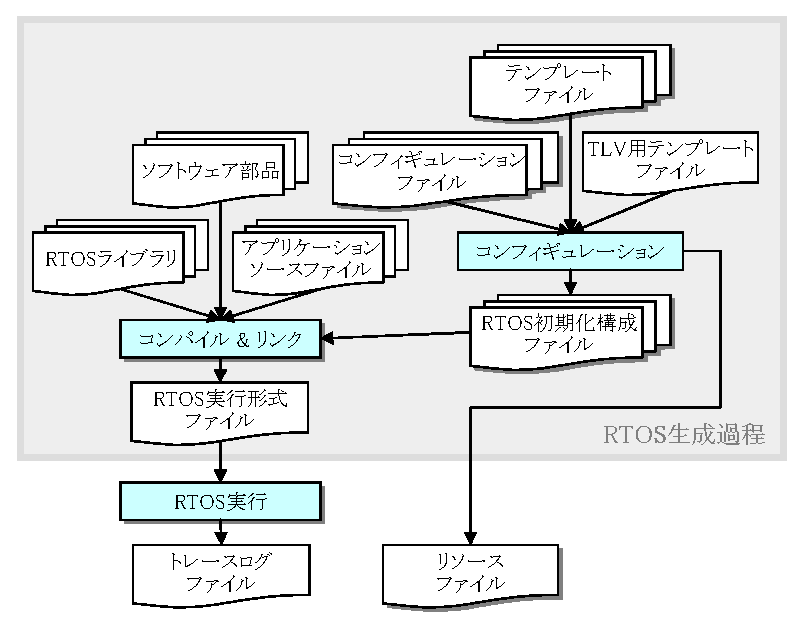
\includegraphics[scale=0.9]{img/rtosMakeProcess.eps}
\caption{TOPPERS/ASPカーネルにおけるトレースログファイルとリソースファイルの生成過程}
\label{fig:rtosMakeProcess}
\end{center}
\end{figure}

\subsection{実行結果}

TLVでTOPPERS/ASPカーネルのトレースログファイルと,リソースファイルを読み込み,可視化表示した実行結果のスクリーンショットを図\ref{fig:aspTLVscreenShot}に示す.

\begin{figure}[!h]
\begin{center}
\includegraphics[width=15cm]{img/aspTLVscreenShot.eps}
\caption{TOPPERS/ASPカーネルのトレースログを可視化したTLV実行結果のスクリーンショット}
\label{fig:aspTLVscreenShot}
\end{center}
\end{figure}

図\ref{fig:aspTLVscreenShot}より,可視化表示する項目が,想定した可視化表現で描画されていることが確認できる.
たとえば,{\tt Task2}の状態が{\tt RUNNABLE},{\tt RUNNING},{\tt WAITING}と遷移し,状態が{\tt WAITING}なのは,{\tt slp\_tsk}というシステムコールを呼んで自ら待ち状態に遷移したから,ということがわかる.

\section{マルチコアプロセッサ用RTOS対応への拡張}

前小節にて,シングルコアプロセッサ用RTOSである,TOPPERS/ASPカーネルのトレースログを可視化表示できることを確認した.
本小節では,これを拡張し,マルチコアプロセッサ用RTOSである,TOPPERS/FMPカーネルのトレースログの可視化表示を試みる.

TOPPERS/FMPカーネルは,対称型(SMP)またはそれに近いマルチコアプロセッサに対応し,リアルタイム性と柔軟性を両立させたRTOSである.
タスクに対してコア間を移動させるシステムコールを実装しており,アプリケーションレベルで負荷分散を実装することが出来る.
OSが負荷分散を行わないという仕様から,各コアはシングルコアプロセッサのときと同じスケジューリング方式を用いることができるため.リアルタイム性の確保が容易になる.

TOPPERS/FMPカーネルのトレースログの形式は,ASPカーネルのものに,トレースログを記録したプロセッサIDを付与した形式になっている.
表\ref{fmpTraceLogSample}にTOPPERS/FMPカーネルのトレースログの例を示す.

\begin{File}{TOPPERS/FMPカーネルのトレースログの例}{fmpTraceLogSample}
[27526775]:[1]: enter to dly_tsk dlytim=10.
[27527154]:[2]: enter to sns_ctx.
[27527284]:[1]: task 4 becomes WAITING.
[27527390]:[2]: leave to sns_ctx state=0.
[27527518]:[1]: dispatch from task 4.
[27527622]:[2]: enter to get_pid p_prcid=1386100.
[27527714]:[1]: dispatch to task 1.
[27527814]:[2]: leave to get_pid ercd=0. prcid=2
[27528162]:[2]: enter to sns_ctx.
[27528338]:[2]: leave to sns_ctx state=0.
[27528522]:[2]: enter to get_pid p_prcid=1386144.
[27528714]:[2]: leave to get_pid ercd=0. prcid=2
\end{File}

\subsection{可視化表示する項目の追加}
\label{subsec421}

TOPPERS/FMPカーネルのトレースログを可視化するにあたり,可視化表示する項目を追加した.

FMPカーネルは,タスクが複数のコアで実行されるため,タスクがどのプロセッサに所属しているのかを可視化表示することにした.
可視化表現としては,背景を所属プロセッサ毎に色分けすることにした.
ここでは,プロセッサ1に所属している間は薄赤,プロセッサ2に所属している間は薄青とした.

\subsection{リソースヘッダファイルの修正}

所属プロセッサを可視化表現するため,リソースタイプ{\tt Task}に所属プロセッサという属性を追加する必要がある.
TOPPERS/ASPカーネル用のリソースヘッダをコピーし,表\ref{fmpResourceTypeTask}に示すように修正した.
修正内容は,ターゲットを{\tt fmp}としたこと,{\tt Attributes}の定義に{\tt prcId}を追加したことである.

\begin{File}{TOPPERS/FMPカーネル用リソースヘッダファイルの一部}{fmpResourceTypeTask}
{
  "fmp":
  {
    "Task":{
      "DisplayName" :"タスク",
      "Attributes" :{
        "prcId":{
          "VariableType"  :"Number",
          "DisplayName"  :"プロセッサID",
          "AllocationType":"Dynamic",
          "CanGrouping"  :true
        },
        ...
\end{File}

\subsection{変換ルールファイルの修正}

FMPカーネルのトレースログは表\ref{fmpTraceLogFormat}のような形式になっている.

\begin{table}[!h]
\begin{quote}
\begin{breakbox}
{\tt [}{\it time}{\tt ]:[}{\it prcId}{\tt ]: }{\it tracelog}
\end{breakbox}
\caption{TOPPERS/FMPカーネルのトレースログの形式}
\label{fmpTraceLogFormat}
\end{quote}
\end{table}

{\it prcId}がプロセッサIDであり,{\it tracelog}はASPカーネルのトレースログの時刻以降と同じである.

修正内容として,まず,検索対象となるトレースログの正規表現をプロセッサIDを考慮して修正する.
次に,実行状態のタスクを参照しているリソース記述({\tt Task(state==RUNNING)})について,プロセッサIDを条件に追加する.
これは,実行状態のタスクが最大プロセッサの数だけ存在するためである.
ASPカーネル用の変換ルールファイルを元に記述した,FMPカーネル用の変換ルールファイルの一部を表\ref{fmpConvertRule}に示す.

\begin{FileNoQuoteMini}{TOPPERS/FMPカーネル用変換ルールファイルの一部}{fmpConvertRule}
{
  "fmp":
  {
    "\[(?<time>\d+)\]:\[(?<pid>\d+)\]: dispatch to task (?<id>\d+)\." : [
      {
        "$EXIST{[${time}]Task(state==RUNNING && prcId==${pid})}"
          :"[${time}]$RES_NAME{[${time}]Task(state==RUNNING && prcId==${pid})}.state=RUNNABLE"
      },
      "[${time}]$RES_NAME{Task(id==${id})}.state=RUNNING"
    ],
    ...
\end{FileNoQuoteMini}

\subsection{可視化ルールファイルの記述}

ASPカーネル用の可視化ルールファイルは,そのまま用いることが出来る.
これは,可視化ルールファイルがトレースログの形式に依存していないからである.

\ref{subsec421}小節で述べた,所属プロセッサの可視化表示のため,FMPカーネル用に,可視化ルールファイルを追加した.
図\ref{fmpShapes}にTOPPERS/FMPカーネル用の可視化ルールファイルを示す.

\begin{FileNoQuote}{TOPPERS/FMPカーネル用の可視化ルールファイル}{fmpShapes}
{
  "fmp":{
    "VisualizeRules":{
      "taskPrcIdChange":{
        "DisplayName":"所属プロセッサ",
        "Target":"Task",
        "Shapes":{
          "prcIdChangeEvent":{
            "DisplayName":"プロセッサID",
            "When":"${TARGET}.prcId",
            "Figures":{
              "${VAL}==1":"prcIdShapes(ff0000)",
              "${VAL}==2":"prcIdShapes(0000ff)",
              "${VAL}==3":"prcIdShapes(00ff00)",
              "${VAL}==4":"prcIdShapes(ff00ff)"
            }
          }
        }
      }
    },
    "Shapes":{
      "prcIdShapes":[
        {
          "Type":"Rectangle",
          "Location":"0,0",
          "Size":"100%,100%",
          "Fill":"${ARG0}",
          "Alpha":30
        }
      ]
    }
  }
}
\end{FileNoQuote}

図\ref{fmpShapes}の内容は,まず,{\tt Shapes}で{\tt prcIdShapes}という所属プロセッサIDを示す図形を定義している.
表示領域の大きさの四角形で,引数で指定される色を塗りつぶしの色として指定している.
また,{\tt Aplha}で透明度を設定し,薄い色になるようにしている.

次に,{\tt VisualizeRules}で{\tt taskPrcIdChange}という名前で所属プロセッサを表示する可視化ルールを定義している.
イベント期間としてリソースタイプ{\tt Task}の所属プロセッサIDを表す属性{\tt prcId}の変化イベントを指定している.
その際の図形として,{\tt prcIdShapes}を指定し,変化後の所属プロセッサID({\tt prcId})の値で条件分けをして引数に与える色を変えている.
ここでは,プロセッサの数を4つまで対応できるようにした,

\subsection{実行結果}

以上のファイルの修正・追加を行い,TOPPERS/FMPカーネルのトレースログをTLVで可視化した.
図\ref{fig:fmpTLVscreenShot}にスクリーンショットを示す.

\begin{figure}[t]
\begin{center}
\includegraphics[width=15cm]{img/fmpTLVscreenShot.eps}
\caption{TOPPERS/FMPカーネルのトレースログを可視化したTLV実行結果のスクリーンショット}
\label{fig:fmpTLVscreenShot}
\end{center}
\end{figure}

図\ref{fig:fmpTLVscreenShot}より,各タスクの所属プロセッサにより,背景の色が分けて表示されていることがわかる.

\section{組み込みコンポーネントシステムの可視化}



\if0
\section{可視化表示項目の追加・変更}

\begin{figure}[t]
\begin{center}
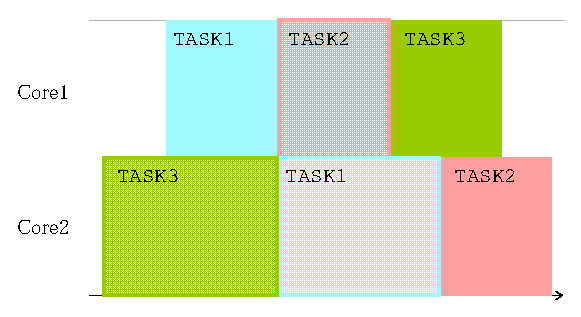
\includegraphics[height=3cm]{img/runningTaskChangeVisual.eps}
\caption{実行タスクの変化の可視化表現例}
\label{fig:runningTaskChangeVisual}
\end{center}
\end{figure}

\begin{figure}[!h]
\begin{center}
\includegraphics[width=15cm]{img/fmpRunTaskTLVscreenShot.eps}
\caption{TOPPERS/FMPカーネルのトレースログで実行タスクの変化を可視化したTLV実行結果のスクリーンショット}
\label{fig:fmppTLVscreenShot}
\end{center}
\end{figure}

実行タスクの変化の可視化表現は,四角形で,上左隅に実行タスク名を文字列を出力するとする.
また,四角形の色を実行タスク毎に変えて出力するとする.
図\ref{fig:runningTaskChangeVisual}に実行タスクの変化の可視化表現の例を示す.
実行タスクの変化を可視化している行では,時間の経過に従い,{\tt Task1},{\tt Task2},{\tt Task3}と実行状態のタスクが変化しているのがわかる.
\fi